%----------------------------------------------------------------------------------------
%	PACKAGES AND THEMES
%----------------------------------------------------------------------------------------
\documentclass[aspectratio=169,xcolor=dvipsnames, t]{beamer}
\usepackage{fontspec} % Allows using custom font. MUST be before loading the theme!
\usetheme{SimplePlusAIC}
\usepackage{hyperref}
\usepackage{graphicx} % Allows including images
\usepackage{booktabs} % Allows the use of \toprule, \midrule and  \bottomrule in tables
\usepackage{svg} %allows using svg figures
\usepackage{tikz}
\usepackage{makecell}
\usepackage{wrapfig}
% ADD YOUR PACKAGES BELOW
\usepackage{subcaption}

%----------------------------------------------------------------------------------------
%	TITLE PAGE CONFIGURATION
%----------------------------------------------------------------------------------------

\title[Markov]{Modèles des langues : Chaînes de Markov} % The short title appears at the bottom of every slide, the full title is only on the title page
\subtitle{Approche probabiliste}

\author{Luis Moreno}
\institute[Sorbonne Université]{UFR de Sociologie et d'Informatique pour les Sciences Humaines 
\newline
Sorbonne Université
}
% Your institution as it will appear on the bottom of every slide, maybe shorthand to save space


\date{\today} % Date, can be changed to a custom date
%----------------------------------------------------------------------------------------
%	PRESENTATION SLIDES
%----------------------------------------------------------------------------------------

\begin{document}

\maketitlepage

\begin{frame}[t]{Agenda}
    % Throughout your presentation, if you choose to use \section{} and \subsection{} commands, these will automatically be printed on this slide as an overview of your presentation
    \tableofcontents
\end{frame}

%------------------------------------------------
% Section divider frame
\makesection{Introduction}

%------------------------------------------------
\begin{frame}{Modèles de Markov}
	\begin{itemize}
		\item Méthode stochastique pour l'étude d’événements aléatoires.
		\item Crée par Andrei Markov, mathématicien russe
		\begin{itemize}
			\item Fondateur de la théorie probabiliste : Processus Stochastiques.
			\item Représentation des processus stochastiques qui analysent la corrélation d'états dans le temps.
		\end{itemize} 
		\item Introduisant la notion de chaîne en 1902
		\item Mieux connu comme \textbf{Chaînes de Markov}
		\item Représenté comme une matrice (\textit{Matrice de confusion} o un graphe)
	\end{itemize}

\end{frame}


%------------------------------------------------
\begin{frame}{Représentations}
	\begin{itemize}
		\item Représenté comme une matrice (\textit{Matrice de confusion MC})
		\begin{itemize}
			\item LA MC sert à indiquer la probabilité d'une transition d'un état à autre.
			\item Chaque position contient la probabilité de passer d'un état à autre.
		\end{itemize} 
		\item ... o un graphe
		\begin{itemize}
			\item Avec des cercles représentant les états,
			\item et des flèches représentant les possibles transition parmi les états.
			\item Les flèches indiquent aussi la probabilité de transition.
		\end{itemize} 
	\end{itemize}
	\begin{figure}
		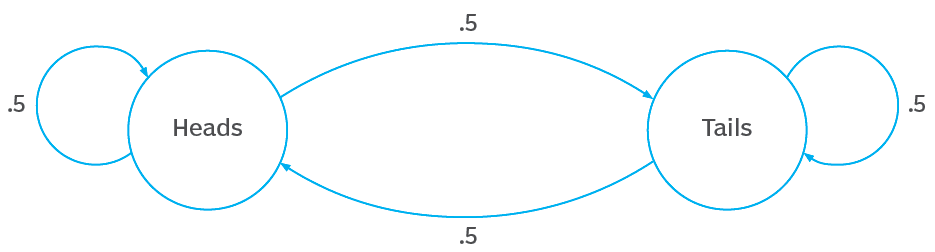
\includegraphics[height=0.25\paperheight]{figures/markov_chain_coin_toss-f.png}
	\end{figure}
	
\end{frame}
%------------------------------------------------

\begin{frame}{Chaînes de Markov}
	
	\begin{columns}
		\begin{column}{0.70\textwidth}
			\begin{enumerate}
				\item Modéliser une séquence d'états.
				\begin{itemize}
					\item Tous les états sont observables
					\item \textcolor{red}{Hidden Markov Models}
				\end{itemize}
				\item Se déplacer à travers les états avec probabilité spécifique.
				\item En constituant donc une chaîne d'états.
			\end{enumerate}
		
			\begin{alertblock}{Important !}
				\begin{itemize}
					\item L'état précédent aura impacté l'état actuel
					\item L'état actuel impactera l'état prochain
				\end{itemize}
			\end{alertblock}			

		\end{column}
		\begin{column}{0.28\textwidth}
			\begin{figure}
				\includegraphics[height=0.6\paperheight ]{figures/markov_exemple.pdf}
			\end{figure}
		\end{column}
	\end{columns}
	

\end{frame}

%------------------------------------------------

\begin{frame}{... un type de modèle de Markov}
	
	
	
	\begin{block}{Génération de textes}
		\begin{itemize}
			\item \textbf{Claude Shannon}\footnote{Considéré comme le père de la Théorie de l'information pour son travail de modélisation de la transmission et réception de l'Information en 1948} a utilisé les chaînes de Markov pour analyser les séquence de caractères de l'anglais.
			\item Comme résultat, il a obtenu un modèle capable de générer de texte en anglais.
			\item ... ses travaux ont boosté le progrès des lignes de recherche comme Linguistique Informatique et Traitement Automatique des Langues.
		\end{itemize}
		
	\end{block}
	
\end{frame}


%------------------------------------------------

\begin{frame}{Algorithmes appliqués au Markov}
	
	\begin{itemize}
		\item \textbf{Algorithme Viterbi} :
		\begin{itemize}
			\item Pour calculer l'état prochain, il considère la séquence (S) la plus récurrente
			\item $S=[currentState, nextState]$
		\end{itemize}
	
		\item \textbf{Algorithme Forward} :
		\begin{itemize}
			\item Calcule la probabilité distributionnelle étant donné une séquence  d'états.
			\item $S=[state_0,..., state_n] , n = $\textit{nombre total d'observations}
		\end{itemize}
	
		\item \textbf{Algorithme Baum-Welch} :
		\begin{itemize}
			\item Estimer les probabilités initiales,
			\item les fonctions de transitions
			\item et les fonctions d'observations
		\end{itemize}
		  
	\end{itemize}
	
\end{frame}


%------------------------------------------------

\begin{frame}{Implémentations}
	
	\begin{itemize}
		\item Préférences des clients / Marketing.
		\item Durabilité des employés / RH.
		\item Fiabilité des machines industrielles.
		\item Futures prix des produits / Finances.
		\item \textbf{TALNE} and \textbf{ML} :
		\begin{itemize}
			\item Génération de texte
			\item Détection d'entités nommées
			\item POS-tagging
			\item Apprentissage par renforcement \textit{Reinforcement learning}
		\end{itemize}
		
		\item \textbf{Santé} :
		\begin{itemize}
			\item Durée des symptômes Covid selon ville
		\end{itemize}
		
	\end{itemize}
	
\end{frame}

%------------------------------------------------
% Section divider frame
\makesection{Quelques exemples}

%------------------------------------------------
% Lists
\begin{frame}{Parking lots ...}
	Nous avons vu l'exemple de Shannon, mais voyons un exemple plus réel...
	\begin{itemize}
		\item Un parking avec un nombre de places disponible
		\item Pour calculer le nombre de places libres, certaines variables doivent être analysées
		\begin{enumerate}
			\item Jour,
			\item Heure dans la journée,
			\item Tarif du parking,
			\item Proximité,
			\item Proximité au travail,
			\item Nombre de places gratuites dans le voisinage.
		\end{enumerate}
	\end{itemize}
\end{frame}


%------------------------------------------------
% Lists
\begin{frame}{Parking lots ...}
	Nous avons vu l'exemple de Shannon, mais voyons un exemple plus réel...
	\begin{itemize}
		\item Un parking avec un nombre de places disponible
		\item Pour calculer le nombre de places libres, certaines variables doivent être analysées
		\begin{enumerate}
			\item \textit{Jour} et 
			\item \textit{heure dans la journée},
			\item \textbf{Tarif du parking},
			\item Proximité,
			\item Proximité au travail,
			\item Nombre de places gratuites dans le voisinage.
		\end{enumerate}
	\end{itemize}
	
	Quelques caractéristiques sont indépendantes; mais pas toutes !
	
\end{frame}

%------------------------------------------------
% Lists
\begin{frame}{Prédictions hypothétiques ... }
	En considérant l'exemple du parking
	\begin{itemize}
		\item Quel sera le taux d'occupation du parking dans 3 heures ?
		\item Quelle est la probabilité que le parking soit rempli à 50 \% puis à 25 \% en 5 heures ?
	\end{itemize}
	
\end{frame}

%------------------------------------------------
% Lists
\begin{frame}{Cas d'étude appliqué}
	Les données suivantes concernent le programme d'entraînement d'une personne X qui souhaite avoir un contrôle de sa performance.
	
	\begin{block}{Routine}
		\begin{itemize}
			\item Run (3 miles)
			\item Push-ups (20)
			\item Rowing (15 minutes)
			\item Pull-ups(20 minutes)
		\end{itemize}
	\end{block}

	\textcolor{red}{La personne X ne suit pas le même ordre de son programme. Mais il y a quand même un pattern observable.}
	
	\textcolor{blue}{Le premier exercice est aléatoire, mais celui-ci impacte dans le prochain exercice.}
	
\end{frame}


%------------------------------------------------
% Lists
\begin{frame}{Cas d'étude appliqué - Problématique}

	X souhaite donc comprendre plus sur comment optimiser son entraînement en considérant l'ordre de sa routine.\\
	
	Et cela peut se faire avec \textbf{Markov} !
	
	\begin{alertblock}{Markov assumption !}
		A Markov chain has short-term memory, it only remembers where you are now and where you want to go next.
	\end{alertblock}
	
\end{frame}


%------------------------------------------------
% Lists
\begin{frame}{Cas d'étude appliqué - hypothèses}
	
	Si vous enregistrez vos séances d'entraînement durant une période suffisante, vous pourriez prédire des comportements intéressants :
	
	\begin{itemize}
		\item Si je commence la séance d'entraînement par une course, quelle est la probabilité que je fasse des pompes lors de la deuxième série ?
		\item Dans une séance d'entraînement en trois séries, quelle est la probabilité que je fasse : 1) de la course, 2) des pompes et 3) des tractions ?
		\item Quelle est la probabilité que je fasse l'un des exercices de la quatrième série ?
	\end{itemize}
	
	
\end{frame}
%------------------------------------------------
% Lists
\begin{frame}{Cas d'étude appliqué - Structuration des données}
	
	Enregistrement des séances pendant N jours.
	\vspace{0.5cm}
	\begin{figure}
		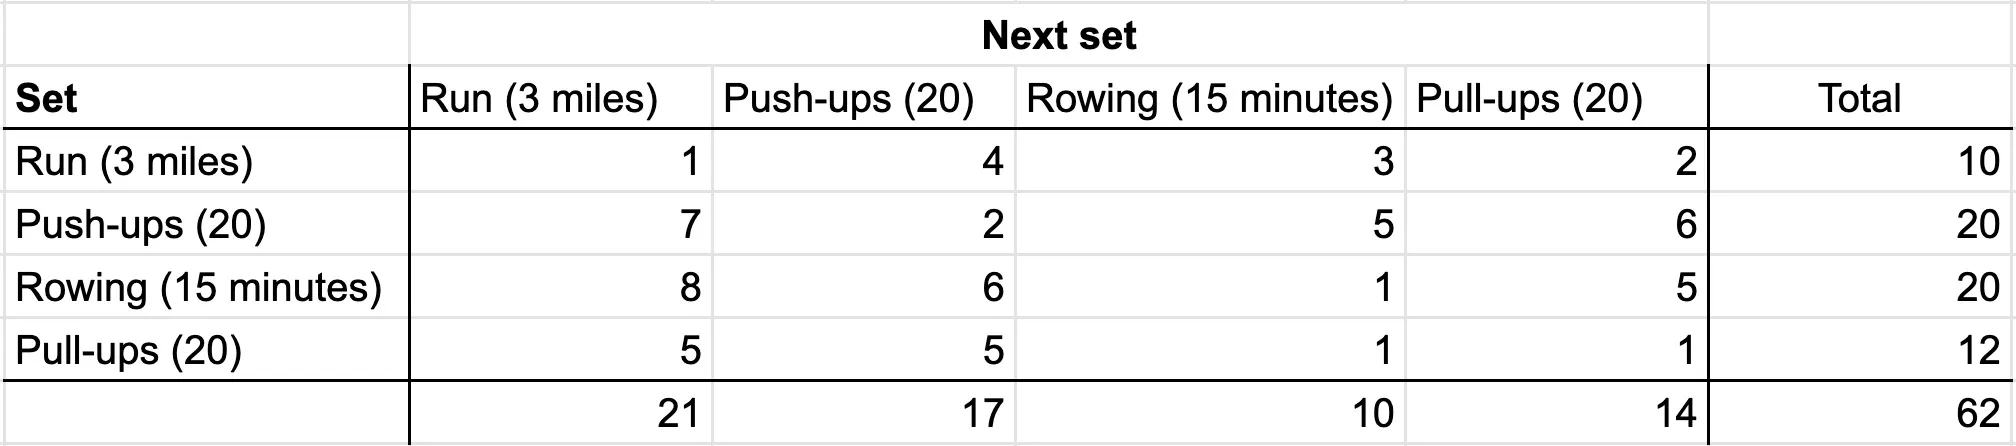
\includegraphics[height=0.35\paperheight]{figures/entrainementLogs.png}
	\end{figure}
	\textcolor{red}{8 fois sur 20 X a fait une série de 15 minutes d'aviron, la série suivante était une course de 3 miles.}

\end{frame}
%------------------------------------------------
% Lists
\begin{frame}{Cas d'étude appliqué - Codification probabiliste}

Codifier les dépendances entre les états, en utilisant des probabilités conditionnelle -> \textbf{Probabilité de transition}.

\begin{figure}
	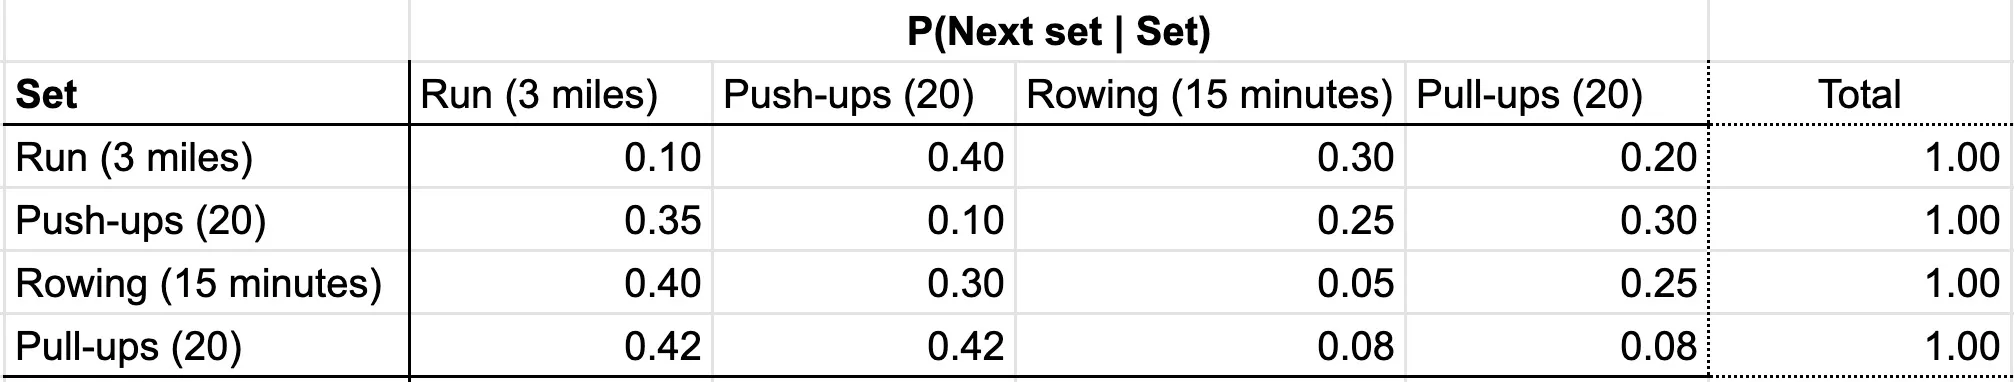
\includegraphics[height=0.3\paperheight]{figures/entrainementLogsEnconded.png}
\end{figure}

1. Si je commence la séance d'entraînement par une course, quelle est la probabilité que je fasse des pompes lors de la deuxième série ?


\end{frame}

%------------------------------------------------
% Lists
\begin{frame}{Cas d'étude appliqué - Codification probabiliste}
	
	1. Si je commence la séance d'entraînement par une course, quelle est la probabilité que je fasse des pompes lors de la deuxième série ?

	\begin{figure}
		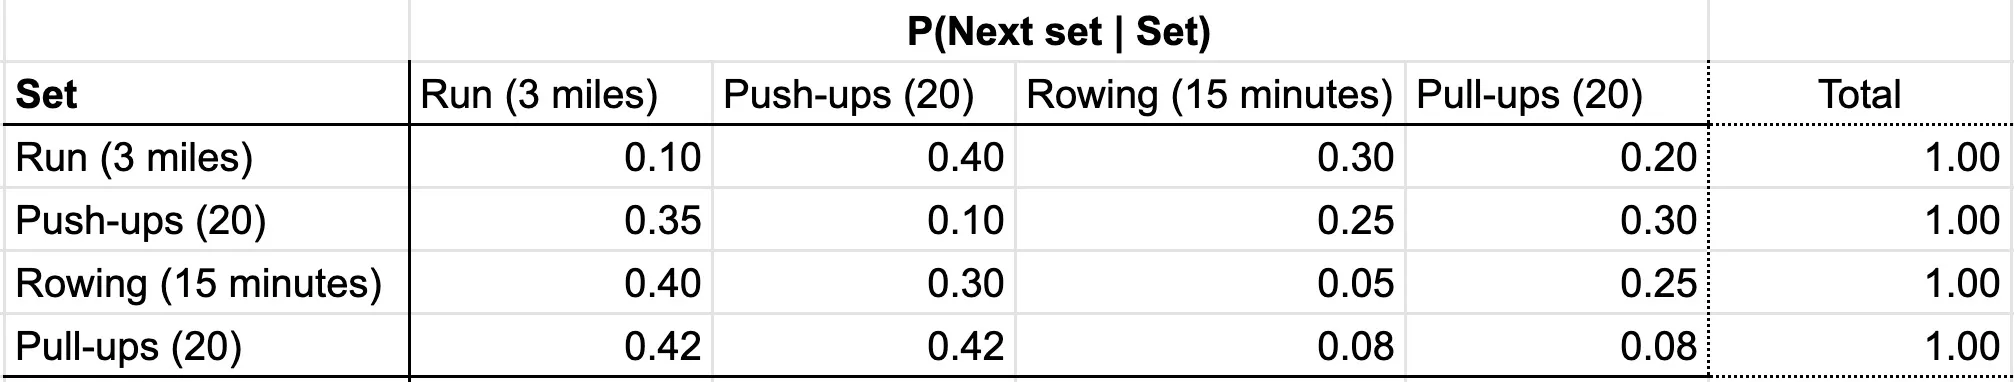
\includegraphics[height=0.3\paperheight]{figures/entrainementLogsEnconded.png}
	\end{figure}
	\textcolor{red}{La probabilité de faire 20 pompes alors que vous venez de terminer une course de 3 miles est de 40 \%. En effet, P(20 pompes | Course) = 4/10 = 0,4.}
	
\end{frame}

%------------------------------------------------
% Lists
\begin{frame}{Cas d'étude appliqué - Représentation matricielle}
	
	En notation mathématique, ces probabilités peuvent être représentées sous la forme d'une matrice de transition de $4\times4$.
	
	\begin{figure}
		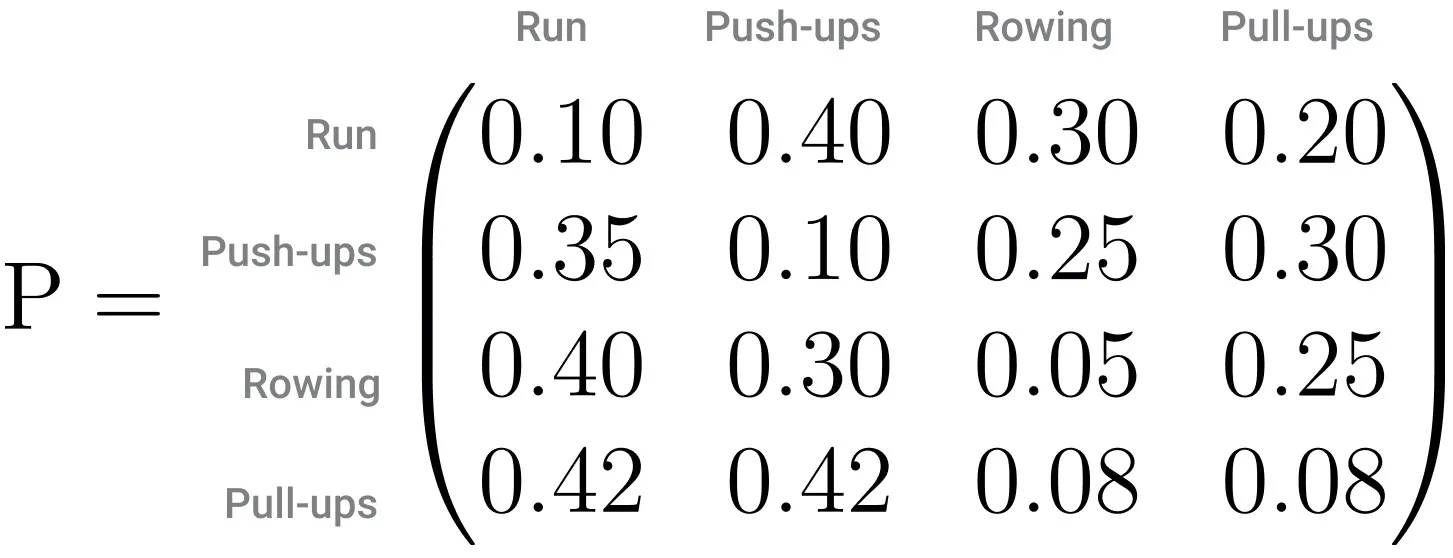
\includegraphics[height=0.4\paperheight]{figures/matriceTransition.png}
	\end{figure}
	
\end{frame}


%------------------------------------------------
% Lists
\begin{frame}{Cas d'étude appliqué - Représentation en graphe}
	
	\begin{figure}
		\centering
		\begin{subfigure}{.5\textwidth}
			\centering
			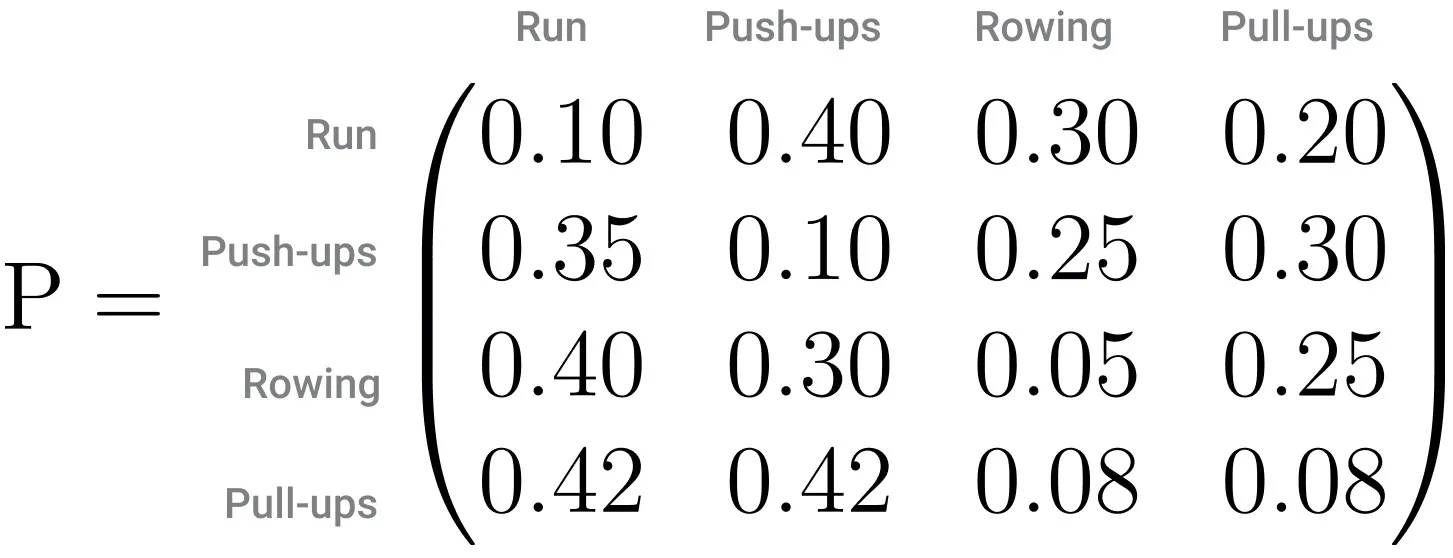
\includegraphics[width=\linewidth]{figures/matriceTransition.png}
			\caption{Matrice de transition}
			\label{fig:sub1}
		\end{subfigure}%
		\begin{subfigure}{.5\textwidth}
			\centering
			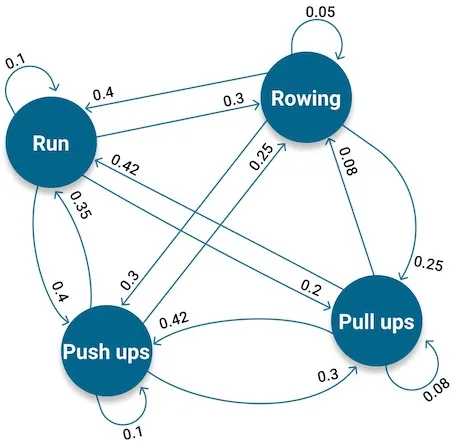
\includegraphics[width=0.7\linewidth]{figures/grapheTransition.png}
			\caption{Graphe de transition}
			\label{fig:sub2}
		\end{subfigure}
		\caption{Représentation communes}
		\label{fig:test}
	\end{figure}
	
\end{frame}


%------------------------------------------------
% Lists
\begin{frame}{Cas d'étude appliqué}
	
	
	\begin{block}{Points à considérer}
		\begin{itemize}
			\item état initial
			\item état finale
			\item \textbf{Time-frame} : nb d'étapes pour aller de l'état initial à l'état final
		\end{itemize}
	\end{block}
	
	\begin{examples}
		Si l'état de départ est de courir 3 miles, parce que c'est ainsi que vous avez choisi de commencer, et l'état final est une série de 20 pompes. Comme vous faites des prédictions pour la deuxième série d'exercices, le time-frame est de 2.
	\end{examples}
	
\end{frame}

%------------------------------------------------
% Lists
\begin{frame}{Cas d'étude appliqué}
	
	Ensuite, calculer la probabilité totale. 
	Combiner tous les chemins dans la chaîne de Markov, où on commence par une course suivi par une série des pompes en deux étapes temporelles.
	\vspace{0.5cm}
	\begin{enumerate}
		\item Go for run given that you’ve just completed a run, then do a set of push-ups.
		\begin{itemize}
			\item $P_{run,run}*P_{push-ups,run}$
		\end{itemize}
		\item Do 20 push-ups given that you’ve just completed a run, then do another set of push-ups.
			\begin{itemize}
			\item $P_{push-ups,run}*P_{push-ups,push-ups}$
			\end{itemize}
		\item Row for 15 minutes given that you’ve just completed a run, then do 20 push-ups.
			\begin{itemize}
			\item $P_{rowing,run}*P_{push-ups,rowing}$
			\end{itemize}
		\item Do 20 pull-ups given that you’ve just completed a run, then do 20 push-ups.
			\begin{itemize}
			\item $P_{pull-ups,run}*P_{push-ups,pull-ups}$
			\end{itemize}
	\end{enumerate}
	
\end{frame}

%------------------------------------------------
% Lists
\begin{frame}{Cas d'étude appliqué}
	Si l'on considère l'ensemble des chemins, la probabilité d'effectuer une séance d'entraînement en deux temps, où l'on commence par une course et où l'on termine par des pompes, est de 25 \%.
	
	\begin{figure}
		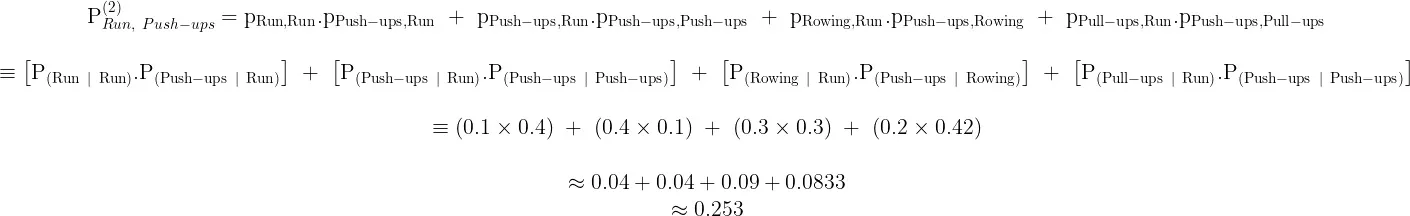
\includegraphics[height=0.25\paperheight]{figures/equiationiGeneral.png}
	\end{figure}
	
\end{frame}


%------------------------------------------------
% Section divider frame
\makesection{Questions ?!}

%------------------------------------------------
% Section divider frame
\makesection{TD-1 ! Classification de textes}


%------------------------------------------------
% Lists
\begin{frame}{Classificateur}
	\begin{itemize}
		\item Question ... 
		\item Étant donné un poème, pouvons-nous savoir à quel auteur il appartient ?
		\item Input(texte) -> Classifier() --> est-ce que c'est un poème d'Allan Poe ?
	\end{itemize}

	\vspace{0.5cm}
	
	\textbf{Autres exemples}	
	\begin{itemize}
		\item E-mail
		\begin{itemize}
			\item Spam or not spam
		\end{itemize}
		\item Critique d'un film
		\begin{itemize}
			\item Positif ou négatif 
		\end{itemize}
	\end{itemize}
	
\end{frame}

%------------------------------------------------
% Lists
\begin{frame}{Problématique}
	\begin{itemize}
		\item Classification de textes, une tâche des méthodes non supervisées
		\item Markov tolère que de texte, pas d’étiquettes.
		\item Comment résoudre le problème ?
			\begin{itemize}
				\item \textbf{Naïve Bayes}
				\item ... Building a Bayes classifier based on rules
			\end{itemize}
	\end{itemize}
	
	\begin{figure}
		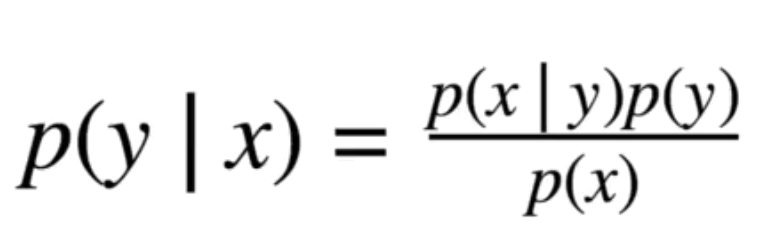
\includegraphics[height=0.25\paperheight]{figures/eq1.png}
	\end{figure}
	
\end{frame}

%------------------------------------------------
% Lists
\begin{frame}{Étape d'entraînement - $A$ et $\pi$ }
	\begin{itemize}
		\item Entraîner les modèles linguistiques nécessaires ... une par Classe.
		\begin{itemize}
			\item Définir et calculer $A$ et $\pi$ 
			\item ... Building a Bayes classifier based on rules
		\end{itemize}
		\item À partir de $A$ et $\pi$, et une séquence ${s_1,s_2,...s_T}$. Quelle est la probabilité de trouver cette séquence ?
		
		\item Comment calculer $A$ et $\pi$ ?
	\end{itemize}
	
	\begin{figure}
		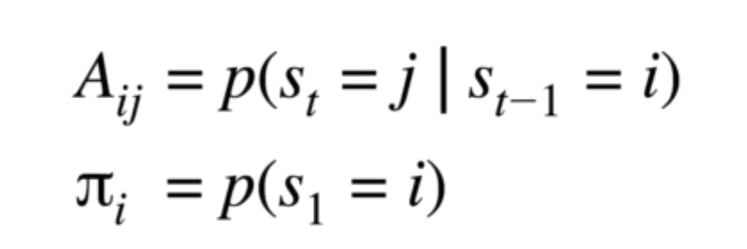
\includegraphics[height=0.25\paperheight]{figures/eq1AnPi.png}
	\end{figure}
	
\end{frame}



%------------------------------------------------
% Lists
\begin{frame}{Étape d'entraînement - les séquences}
	\begin{itemize}
		\item Entraîner les modèles linguistiques nécessaires ... une par Classe.
		\begin{itemize}
			\item Définir et calculer $A$ et $\pi$ 
			\item ... Building a Bayes classifier based on rules
		\end{itemize}
		\item \textbf{ À partir de $A$ et $\pi$, et une séquence ${s_1,s_2,...s_T}$. Quelle est la probabilité de trouver cette séquence ?}
	\end{itemize}
	
	\begin{figure}
		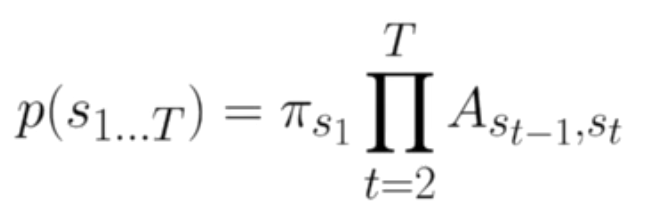
\includegraphics[height=0.2\paperheight]{figures/eqSeqMult.png}
	\end{figure}
	
	\begin{itemize}
		\item C'est que la multiplication des valeurs des transitions calculées.
		\item Si une de ces valeurs est $0$ ? Une transition jamais vue.
		\item Tout devient $0$
	\end{itemize}
	
\end{frame}

%------------------------------------------------
% Lists
\begin{frame}{Étape d'entraînement - $\hat{A}$ et $\hat{\pi}$}
	\begin{itemize}
		\item Entraîner les modèles linguistiques nécessaires ... une par Classe.
		\begin{itemize}
			\item Définir et calculer $A$ et $\pi$ 
			\item ... Building a Bayes classifier based on rules
		\end{itemize}
		\item À partir de $A$ et $\pi$, et une séquence ${s_1,s_2,...s_T}$. Quelle est la probabilité de trouver cette séquence ?
		
		\item \textbf{Comment lisser  $A$ et $\pi$ ?}
	\end{itemize}

	\begin{figure}
		\centering
		\begin{subfigure}{.5\textwidth}
			\centering
			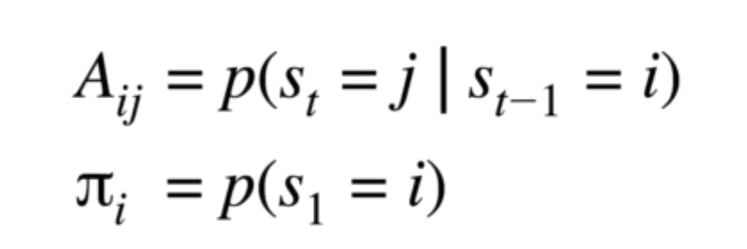
\includegraphics[width=0.78\linewidth]{figures/eq1AnPi.png}
			\caption{Version classique}
		\end{subfigure}%
		\begin{subfigure}{.5\textwidth}
			\centering
				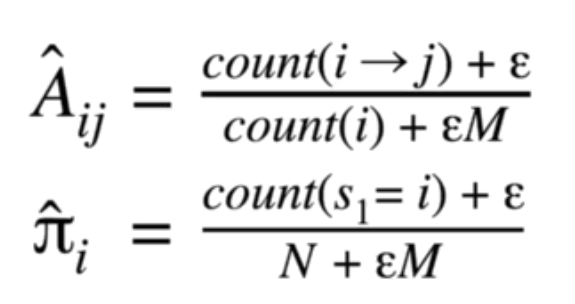
\includegraphics[width=0.48\paperheight]{figures/eq1AnPiEst.png}
			\caption{Estimation de $A$ et $\pi$}
		\end{subfigure}
	\end{figure}
	
\end{frame}


%------------------------------------------------
% Lists
\begin{frame}{Étape d'entraînement - smoothing}
	\begin{itemize}
		\item Entraîner les modèles linguistiques nécessaires ... une par Classe.
		\begin{itemize}
			\item Définir et calculer $A$ et $\pi$ 
			\item ... Building a Bayes classifier based on rules
		\end{itemize}
	\end{itemize}
	
	\begin{figure}
		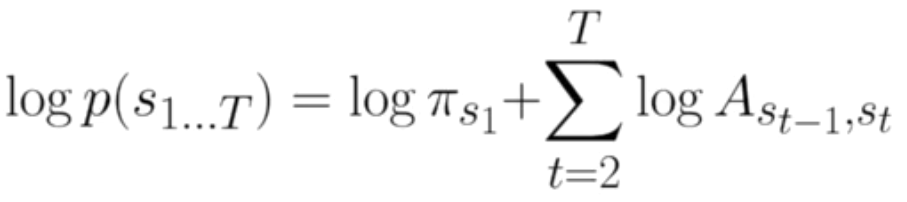
\includegraphics[height=0.2\paperheight]{figures/eqSmoothed.png}
	\end{figure}

	\begin{itemize}
		\item Nous remplaçons la multiplication pour somme (Simplification)
		\item On garde que les logged values car arg max needed
		\item Respectez l'ordre : log() and then sum()
	\end{itemize}
	
\end{frame}

%------------------------------------------------
% Lists
\begin{frame}{Fonctionnement}
\begin{itemize}
	\item Étant donné les objets $A$ et $\pi$ et un texte comme input
	\item ... calculer la probabilité que ce texte appartienne a la classe analysée
\end{itemize}

\begin{figure}
	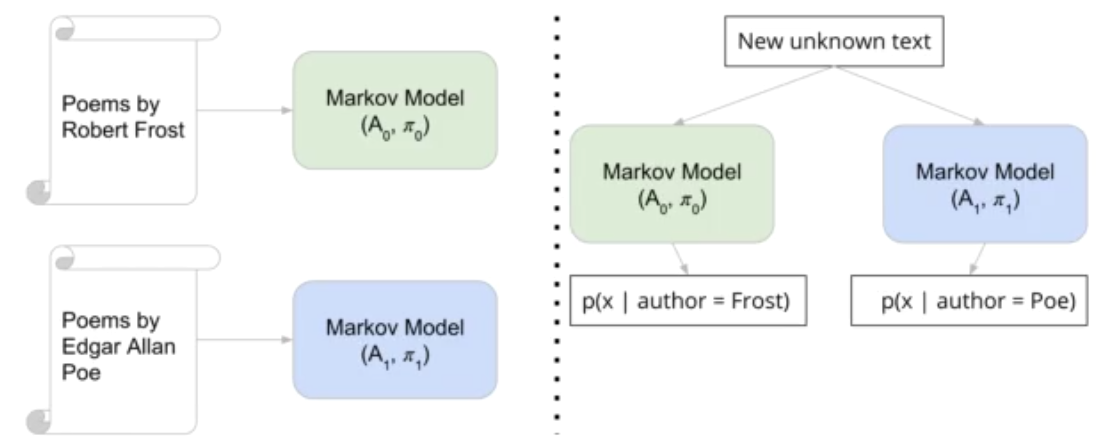
\includegraphics[height=0.5\paperheight]{figures/img1.png}
\end{figure}


\end{frame}

%------------------------------------------------
% Lists
\begin{frame}{Les règles...}
	\begin{itemize}
		\item On a \textit{p(poème|auteur)} mais on a besoin de \textbf{\textit{p(auteur|poème)}}
		\item Nous devons donc appliquer l'équation :
	\end{itemize}
	
	\begin{figure}
		\centering
		\begin{subfigure}{.5\textwidth}
			\centering
			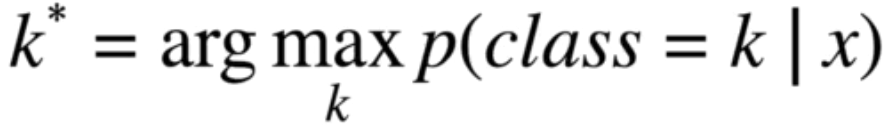
\includegraphics[width=0.7\textwidth]{figures/eq2.png}
		\end{subfigure}%
		\begin{subfigure}{.5\textwidth}
			\centering
			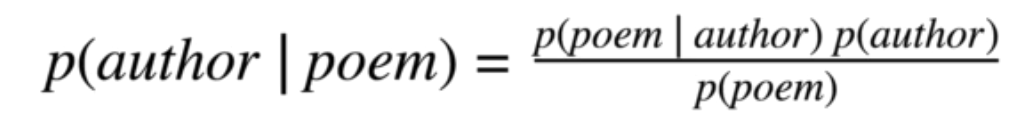
\includegraphics[width=0.8\textwidth]{figures/eq3.png}
		\end{subfigure}
		\textbf{Si l'on simplifie l'équation}
		\begin{figure}
			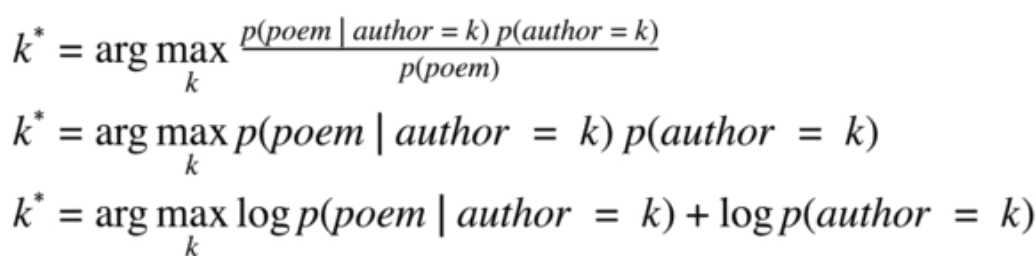
\includegraphics[width=0.7\textwidth]{figures/img2.png}
		\end{figure}
	\end{figure}

\end{frame}



%------------------------------------------------
% Section divider frame
\makesection{TD-2 ! Génération de textes}

%------------------------------------------------

%------------------------------------------------
% Lists
\begin{frame}{Modèle génératif}
	\begin{itemize}
		\item Classification de textes : supervisé (étiquettes)
		\begin{itemize}
			\item Discriminatif
			\item $p(y|x)$
		\end{itemize}
		\item Générateur de textes : non supervisé (pas d'étiquettes)		\begin{itemize}
			\item Génératif
			\item $p(x|y)$
		\end{itemize}
			
	\end{itemize}		
\end{frame}


\begin{frame}{\textit{Sampling} ... }
	\begin{itemize}
		\item Sampling avec N(0,1) : \textit{np.random.randn()}
		\item Sampling avec Bernouli : \textit{np.random.choice([0,1])}
		\item Bernouli avec p(heads=0.8) (où heads = 1) :
		\begin{itemize}
			\item \textit{np.random.choise([0,1] , p=[0.2 , 0.8])}
		\end{itemize} 
	\end{itemize}
	\vspace{0.5cm}
	\textbf{Sampling words} - Supposons que nous avons un vocabulaire = ('cat', 'dog', 'mouse')
	\begin{itemize}
		\item Avec leurs probabilité d'apparition : (0.2, 0.5, 0.3)
		\item Si l'on peut cartographier le vocabulaire  comme (1, 2, 3), ça devient facile
		\begin{itemize}
			\item \textit{np.random.choice(3, p=[0.2, 0.5, 0.3])}
		\end{itemize}
		
	\end{itemize}		
\end{frame}

%------------------------------------------------

\begin{frame}{Problématique}
	Rappelez que le mot prochain dépend uniquement du mot précédent
	\begin{examples}
		\begin{enumerate}
			\item Je me suis préparé moi-même un sandwich au beurre.
			\item Je vais aller lui rendre visite moi-même.
		\end{enumerate}
		\begin{itemize}
			\item \textbf{ Je vais aller lui rendre visite moi-même un sandwich au beurre.}
		\end{itemize}
	\end{examples}

	\begin{examples}
		\begin{enumerate}
			\item Je me suis préparé moi-même un sandwich au beurre.
			\item Le beurre n'est pas une noisette
		\end{enumerate}
		\begin{itemize}
			\item \textbf{ Je me suis préparé moi-même un sandwich au beurre n'est pas une noisette.}
		\end{itemize}
	\end{examples}
\end{frame}
%------------------------------------------------

\begin{frame}{Prolongement du modèle de Markov}
	
	\begin{itemize}
		\item Au lieu d'observer que le mot précédent : 
		\begin{itemize}
			\item Markov de premier ordre
			\item $p(s_t |s_{t-1}, s_{t-2}, ...) = p(s_t | s_{t-1})$
		\end{itemize}
		\item ...on observe les deux mots précédent
		\begin{itemize}
			\item Markov de premier ordre
			\item $p(s_t |s_{t-1}, s_{t-2}, ...) = p(s_t | s_{t-1}, s_{t-2})$
		\end{itemize}
		\item \textit{Afin de mieux prédire le future, il faut mieux observer le passé}
	\end{itemize}

\end{frame}

%------------------------------------------------

\begin{frame}{Modèle complet}
	
	\begin{itemize}
		\item $ \pi_i = p(s_1 = i)$
		
		\item $ A^{(1)}_{ij} = p(s_2 = j | s_1 = i)$
		
		\item $ A^{(2)}_{ijk} = p(s_t = k | s_{t-1}, s_{t-2} = i)$
	\end{itemize}

\begin{example}
	"The quick brown fox jumps over the lazy dog" \\
	"\textbf{The}" -> $\pi$\\
	"\textcolor{red}{The} \textbf{quick}"-> $A^{(1)}$\\
	"\textcolor{red}{The quick} \textbf{brown} " -> $A^{(2)}$\\
	"The \textcolor{red}{quick brown} \textbf{fox} " -> $A^{(2)}$\\
\end{example}
	
\end{frame}

%------------------------------------------------
% Refenrenced
\begin{frame}{Références}
    % Beamer does not support BibTeX so references must be inserted manually as below
    \footnotesize{
        \begin{thebibliography}{99}
            \bibitem[Bento, 2020]{p1} Carolina Bento (2020)
            \newblock Markov models and Markov chains explained in real life: probabilistic workout routine
            \newblock \href{https://towardsdatascience.com/markov-models-and-markov-chains-explained-in-real-life-probabilistic-workout-routine-65e47b5c9a73}{https://towardsdatascience.com/markov-models-and-markov-chains-explained...}
            
            \bibitem[Bento, 2020]{p1} Pat Brans (2022)
            \newblock What is a Markov model?
            \newblock \url{https://www.techtarget.com/whatis/definition/Markov-model}

            \bibitem[Bento, 2020]{p1} Wikipedia free encyclopedia (2024)
            \newblock Markov model
            \newblock \url{https://en.wikipedia.org/wiki/Markov_model}
            
            %\bibitem[Doe, 2013]{p} Jane Doe (2012)
            %\newblock Title of the publication
            %\newblock \emph{Journal Name} 12(3), 45 -- 678.
        \end{thebibliography}
    }
\end{frame}

%----------------------------------------------------------------------------------------
% Final PAGE
% Set the text that is showed on the final slide
\finalpagetext{Thank you for your attention}
%----------------------------------------------------------------------------------------
\makefinalpage
%----------------------------------------------------------------------------------------
\end{document}